\chapter{Threat Modelling}
\label{chap:threat_model}
Threat modelling is an act of security analysis which aids in discovering potential vulnerabilities in an application or a system before they become threats \citep{threat_model_intro}. This exercise is a crucial step in the Software Development Life Cycle (SDLC), as it helps detect the possible flaws in the system, and suitable mitigation can be applied. Similarly, threat modelling will also be conducted for this project, where an authentication server using OIDC protocol is operated in a cloud environment. The approach that this project will apply to threat modelling is based on Shostack's Four Question Framework \citep{shostack}. The questions focus on the project objectives, what could go wrong there, what mitigations could be applied, and whether it can be improved. Using Shostacks questions in conjunction with the OWASP threat modelling process, the application, using OpenID Connect in Cloud, can be analysed \citep{owasp_threat_model}. The objective of threat modelling is to identify as many possible risks that are present in the Open ID Connect application running on a cloud. To add further, the modelling performed will be cloud agnostic meaning these identified mitigations can be applied anywhere irrespective to the cloud provider.


\section{Application Information}
To answer the first question about \textit{what are we working on}, this section will describe the application and the different dependencies that this application contains.
\begin{itemize}
    \item \textbf{Application Name:} Multi-tenant App
    \item \textbf{Application Version:} v1.0
    \item \textbf{Description:} This generic authentication and authorisation application utilises OpenID Connect protocols PKCE flow (See Figure \ref{fig:pkce_flow}) in a public cloud environment. This application will be based on multitenant capability, where the users cannot access each other's resources even though they share the same infrastructure and application. This general API would provide the capabilities mentioned in Table \ref{table:threat_model_entry_points}.
  \end{itemize}

\subsection{Entry Points}
\begin{longtable}{|p{3cm}|p{4cm}|p{4cm}|p{4cm}|}
\caption{Threat modelling: Entry Points}
\label{table:threat_model_entry_points}
\hline
\rowcolor{grey!15}
\textbf{Entry Point} & \textbf{Description} & \textbf{Request Parameters} & \textbf{Response Data} \\
\hline
\endfirsthead
\hline
\rowcolor{grey!15}
\textbf{Entry Point} & \textbf{Description} & \textbf{Request Parameters} & \textbf{Response Data} \\
\hline
\endhead
\endfoot
\hline
\endlastfoot

/authorize & Entry point for user authentication.  & 
- client\_id: The client ID of the application \newline 
%- redirect\_uri: URI where the response will be sent \newline
- scope: Scopes for requested authentication (e.g., OpenID, email) \newline 
- response\_type: Indicates the desired authorization flow (e.g., code) & 
- The authorisation code is to be exchanged for tokens. \newline 
- Error in case of invalid request \\
\hline

/token & Entry point for exchanging authorization code for tokens (access token, ID token, refresh token). & 
- grant\_type: "authorization\_code" \newline 
- code: Authorization code received from /authorize \newline
- redirect\_uri: Must match the original redirect URI used in /login \newline 
- client\_id: The client ID of the application
- code\_verifier: Code used to validate code\_challenge& 
- access\_token: Token for accessing protected resources \newline 
- id\_token: Token containing user identity information \newline 
- Error in case of invalid request \\
\hline

/userinfo & Entry point to retrieve user information using an access token. & 
- access\_token: Token obtained from /token endpoint & 
- id: Unique identifier of the user \newline 
- email: User's email address \newline 
- name: User's full name \newline 
- Error in case of invalid token or request \\
\hline

/logout & Entry point for logging out the user and invalidating tokens. & 
- post\_logout\_redirect\_uri: URI to redirect after successful logout & 
- Redirect to post\_logout\_redirect\_uri \newline 
- Error in case of invalid token or request \\
\hline

\end{longtable}

\begin{longtable}{|p{8cm}|p{8cm}|}
\caption{Threat modelling: Asset Descriptions}
\label{table:threat_model_assets}
\hline
\rowcolor{grey!15}
\textbf{Assets} & \textbf{Description} \\
\hline
\endfirsthead

\hline
\rowcolor{grey!15}
\textbf{Assets} & \textbf{Description} \\
\hline
\endhead

% Assets for PKCE App in Cloud with Multiple Tenants
OAuth Tokens & Used to authorize access to resources on behalf of the user. \\
\hline
User Credentials & Sensitive information (e.g., usernames, passwords) used to authenticate users; protection. \\
\hline
OAuth Authorization Codes & Temporary codes exchanged during OAuth flows are essential for secure authorization in PKCE flows. \\
\hline
Cloud Infrastructure & The underlying infrastructure (servers, storage, networking) that supports the application in the cloud \\
\hline
Application Data & Data created, stored, or processed by the application, which could include user data or system configurations \\
\hline
API Endpoints & Points of interaction where the application exposes functionality to clients See the entry point (Table \ref{table:threat_model_entry_points}). \\
\hline

\end{longtable}


\section{STRIDE Model}
Using the given entry points and assets that the application uses, we can create a level zero Data Flow Diagram (DFD) (See Figure \ref{fig:dfd_app}). This diagram depicts the overview of the entire system with its significant processes, data flow and credential stores. With the help of Figure \ref{fig:dfd_app}, an abstract view of the entire system shows the processes and their relationships that can be used in established threat modelling techniques, namely STRIDE \citep{dfd_stride}. STRIDE is a threat modelling framework used to classify security threats developed by Microsoft \citep{stride_usage}. The letters in the acronym are Spoofing, Tampering, Repudiation, Information disclosure, Denial of service, and Elevation of privilege. The threat categories will be analyzed during the threat modelling \citep{stride}. Using the DFD, a STRIDE threat modelling is carried out, which provides an analysis of some threats in the given context of this model. This threat modelling framework is chosen because it allows for a systematic and structured approach to identify threats in different areas denoted by the acronym and is easy to apply.



\begin{figure}[h!]
\centering
\caption{Data Flow Diagram Level 0 OIDC App}\label{fig:dfd_app}
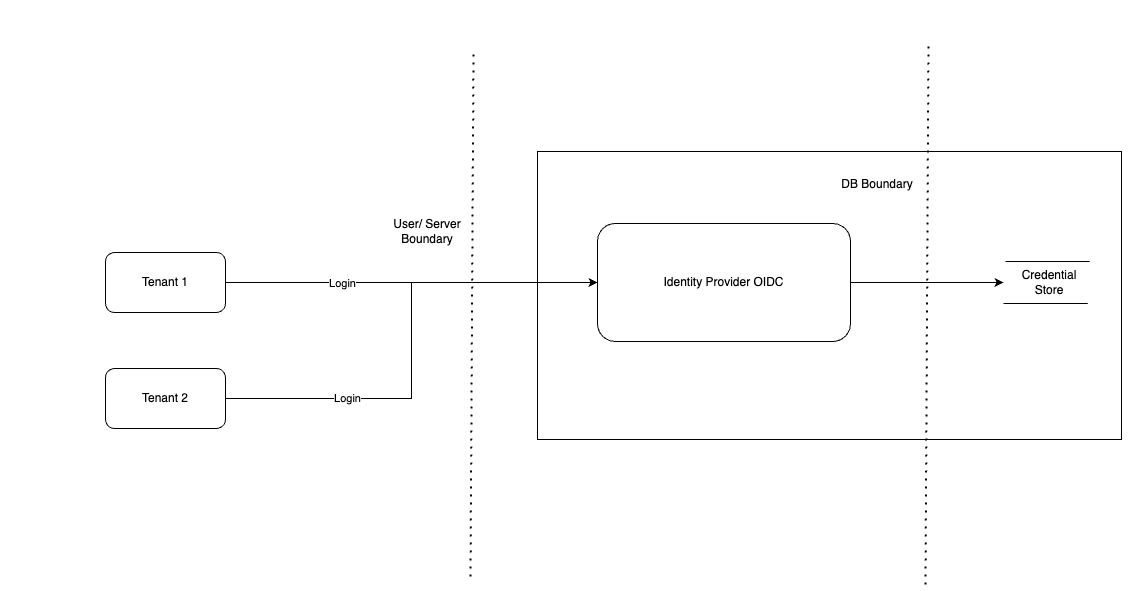
\includegraphics[width=\textwidth, height=320px]{pics/DFD_APP.png}
\end{figure}



\subsection*{1. Spoofing}
\begin{itemize}
    \item \textbf{Threat}: An attacker attempts to impersonate a legitimate user or tenant to gain unauthorised access.
    \item \textbf{Specific Attacks}:
    \begin{itemize}
        \item \textbf{ID Spoofing}: The attacker tries impersonating an End user from another OpenID Provider by using spoofed tokens or changing the token's contents \citep{oidc_attacks}.
        \item \textbf{Credential Stuffing}: Using leaked credentials from other services to gain unauthorised access.
        \item \textbf{Phishing}: Tricking users into providing their credentials through fraudulent login pages. For example, the attackers can manipulate the redirect endpoints to redirect to the malicious URL \citep{open_redirect_oidc_threat}.
        \item \textbf{Man-in-the-Middle Attack (MITM)}: Intercepting the authorization code during the OAuth2 flow.
    \end{itemize}
    \item \textbf{Mitigation}:
    \begin{itemize}
        \item Signed tokens should always be verified at the issuer's end so that a spoofed token cannot bypass the security.
        \item The client should validate the audience and issuer claims to prevent tokens from being used across different services.
        \item Enforce multi-factor authentication (MFA) to prevent credential-based attacks.
        \item PKCE mitigates MITM attacks by tying the authorization code to a unique challenge/response.
        \item Use OAuth2’s \texttt{nonce} and \texttt{state} parameters to protect against replay attacks.
    \end{itemize}
\end{itemize}

\subsection*{2. Tampering}
\begin{itemize}
    \item \textbf{Threat}: Unauthorized modification of data or code during transmission or at rest.
    \item \textbf{Specific Attacks}:
    \begin{itemize}
        \item \textbf{Token Tampering}: This attack targets access, ID, and refresh tokens. Where the attacker manipulates the tokens to add their claims and scopes to allow authorised access \citep{oidc_attacks}.
        \item \textbf{Code Injection}: Injecting malicious code or tokens into the OAuth2 flow.
        \item \textbf{OAuth Token Replay}: Reusing an old token after invalidating or expired.
        \item \textbf{Malicious Endpoint} The discovery endpoints of OIDC, such as the ./wellknown, are tampered with, and malicious endpoints are added to the public endpoint where the attacker can now get sensitive information, as the endpoints are fake \citep{oidc_attacks}.
        \item \textbf{Ransomware}: Unlike just OIDC, cloud technologies, especially public clouds, are susceptible to ransomware attacks. In this attack, the attacker tries to misuse existing vulnerabilities and steal sensitive data or encrypt them, making them unusable \citep{ransomeware}.
    \end{itemize}
    \item \textbf{Mitigation}:
    \begin{itemize}
         \item A key should always sign the tokens like ID tokens containing user information and must be verified each time with the issuer when used.
        \item Use PKCE to prevent authorization code injection by requiring a code challenge.
        \item Sign and validate JWT tokens to ensure integrity and detect tampering.
        \item Implement token expiration and invalidation mechanisms and rotating refresh tokens to reduce token reuse.
        \item Use different tools to detect anomalies in the system and prevent malware such as ransomware from propagating deep into different services into the cloud \citep{ransomeware}.
        \item Perform network segregation and build zero privilege systems to allow only the required actors to access the services and no more \citep{zero_trust}. 
    \end{itemize}
\end{itemize}

\subsection*{3. Repudiation}
\begin{itemize}
    \item \textbf{Threat}: Users or tenants could deny performing certain actions, making it difficult to establish accountability.
    \item \textbf{Specific Attacks}:
    \begin{itemize}
        \item \textbf{Action Denial}: A malicious tenant denies having issued a token or performed an action within the application that could deny sending or receiving messages in a digital transaction \citep{repudiation}.
        \item \textbf{Tenant Switching}: Similarly, in a multi-tenant environment, a user might gain access to another tenant’s data and deny the action.
    \end{itemize}
    \item \textbf{Mitigation}:
    \begin{itemize}
        \item Use signed access tokens (JWT) with non-repudiation attributes.
        \item Log every critical action and tenant interaction, including token issuance and API calls, with cryptographically signed entries.
        \item Use immutable logs with encryption.
    \end{itemize}
\end{itemize}

\subsection*{4. Information Disclosure}
\begin{itemize}
    \item \textbf{Threat}: Sensitive data such as access tokens, personal data, or tenant-specific information is exposed.
    \item \textbf{Specific Attacks}:
    \begin{itemize}
        \item \textbf{Cross-Tenant Data Leakage}: Improper multi-tenant isolation could make one tenant’s data accessible to another.
        \item \textbf{Token Exposure}: OAuth2 tokens might be leaked through insecure communication.
        \item \textbf{Cloud Misconfigurations}: Misconfigured database leading to data exposure.
    \end{itemize}
    \item \textbf{Mitigation}:
    \begin{itemize}
        \item Implement strong tenant isolation at the application and database levels, ensuring no cross-tenant data leakage.
        \item Use end-to-end encryption and enforce HTTPS for all communications.
        \item Conduct regular security audits to identify cloud misconfigurations.
        \item Manage whitelisted redirect URIs and limit callback URLs to trusted domains.
    \end{itemize}
\end{itemize}

\subsection*{5. Denial of Service (DoS)}
\begin{itemize}
    \item \textbf{Threat}: An attacker may overwhelm the service, making it unavailable for legitimate users and tenants.
    \item \textbf{Specific Attacks}:
    \begin{itemize}
        \item \textbf{Token Bombing}: Repeatedly requesting tokens using valid credentials to overload the authorization server.
        \item \textbf{API Rate Limiting Attack}: Flooding API endpoints with excessive requests, leading to resource exhaustion.
        \item \textbf{Resource Starvation}: Exploiting vulnerabilities to consume cloud resources, like CPU or memory, disrupting multi-tenant services.
    \end{itemize}
    \item \textbf{Mitigation}:
    \begin{itemize}
        \item Implement API rate limiting and token request throttling to prevent token bombing.
        \item Use distributed denial of service (DDoS) protection services, such as AWS Shield \citep{aws_shield}.
        \item Ensure each tenant has isolated resource pools to avoid one tenant's traffic affecting others.
        \item Implement service quotas for resource consumption per tenant.
    \end{itemize}
\end{itemize}

\subsection*{6. Elevation of Privilege}
\begin{itemize}
    \item \textbf{Threat}: An attacker could gain higher privileges than authorised, allowing access to sensitive data or functionality.
    \item \textbf{Specific Attacks}:
    \begin{itemize}
        \item \textbf{PKCE Downgrade Attack}: The attacker can remove \texttt{code\_challenge} from the request if the authentication server does not validate the \texttt{code\_verifier}, the token will be issued, allowing unauthorised access \citep{oidc_attacks}.
        \item \textbf{Insecure Multi-Tenant Access Control}: A user accessing other tenants' resources through misconfigured roles or policies.
    \end{itemize}
    \item \textbf{Mitigation}:
    \begin{itemize}
        \item The \texttt{code\_verifier} must be verified at the authentication server and the \texttt{code\_challenge} should be bound the the authorisation code \citep{oidc_attacks}.
        \item Regularly audit role assignments, permissions, and token scopes to detect misconfigurations.
        \item Implement tenant-aware access control to ensure that users can only interact with resources belonging to their tenant.
    \end{itemize}
\end{itemize}
